% NP-Hardness Part 3 -- Metropolis beamer slides
% Compile: pdflatex np-hardness-part-3.tex (x2)
\documentclass[10pt,aspectratio=169]{beamer}

\usetheme{metropolis}
\metroset{block=fill, numbering=fraction, progressbar=frametitle}

\usepackage[T1]{fontenc}
\usepackage{amsmath, amssymb}
\usepackage{booktabs}
\usepackage{tikz}
\usetikzlibrary{arrows.meta, positioning, calc}

% ---- colors -------------------------------------------------------------
\definecolor{mLightBlue}{HTML}{4C72B0}
\definecolor{mGreen}{HTML}{55A868}
\definecolor{mRed}{HTML}{C44E52}
\definecolor{mGray}{HTML}{BFBFBF}
\definecolor{mOrange}{HTML}{DD8452}
\setbeamercolor{alerted text}{fg=mRed}

% ---- helpers ------------------------------------------------------------
\tikzset{
  vtx/.style={draw, circle, minimum size=7mm, inner sep=0pt, font=\small,
              fill=white},
  pick/.style={vtx, fill=mOrange!55},
  cov/.style={vtx, fill=mLightBlue!40},
  edg/.style={thick, mGray!80!black},
  hot/.style={line width=2pt, mOrange},
  box/.style={draw, thick, rounded corners=3pt, minimum height=7mm,
              minimum width=26mm, align=center, font=\small},
  arr/.style={thick, -{Stealth[length=2.5mm]}},
  % overlay-aware keys: onslide=<2->{pick}
  onslide/.code args={<#1>#2}{\only<#1>{\pgfkeysalso{#2}}},
}

% Five vertices on a pentagon, used for G and its complement
\newcommand{\pentagon}[5]{%
  \node[#1] (v1) at (90:1.6)  {1};
  \node[#2] (v2) at (18:1.6)  {2};
  \node[#3] (v3) at (-54:1.6) {3};
  \node[#4] (v4) at (-126:1.6) {4};
  \node[#5] (v5) at (162:1.6) {5};
}

% ---- title --------------------------------------------------------------
\title{NP-Hardness, Part 3}
\subtitle{Clique, Vertex Cover}
\date{}
\author{}

\begin{document}

\maketitle

% =========================================================================
\begin{frame}{Recap}
  To show a problem $B$ is NP-complete:
  \begin{enumerate}
    \item $B \in \mathbf{NP}$: a certificate and a polynomial-time verifier;
    \item a reduction $A \le_p B$ from a known NP-complete $A$.
  \end{enumerate}

  \bigskip
  So far:
  \begin{center}
  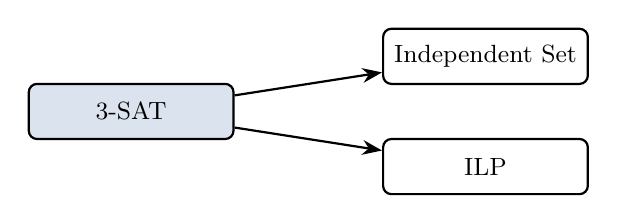
\begin{tikzpicture}
    \node[box, fill=mLightBlue!20] (sat) at (0,0) {3-SAT};
    \node[box] (is) at (4.5,0.7) {Independent Set};
    \node[box] (ilp) at (4.5,-0.7) {ILP};
    \draw[arr] (sat) -- (is);
    \draw[arr] (sat) -- (ilp);
  \end{tikzpicture}
  \end{center}

  \bigskip
  Today: two problems closely related to Independent Set. Each reduction is
  a one-line transformation of the graph.
\end{frame}

% =========================================================================
\section{Clique}

\begin{frame}{Clique}
  A \alert{clique} in $G = (V, E)$ is a set $S \subseteq V$ in which
  \emph{every} pair of vertices is joined by an edge.

  \begin{columns}[c]
    \begin{column}{0.5\textwidth}
      \begin{block}{Clique}
        Given $G$ and $k$, does $G$ have a clique of size $\ge k$?
      \end{block}

      \medskip
      \textbf{In NP.} Certificate: the set $S$. Check $|S| \ge k$ and all
      $\binom{|S|}{2}$ pairs, $O(n^2)$ time with an adjacency matrix.
    \end{column}
    \begin{column}{0.45\textwidth}
      \begin{center}
      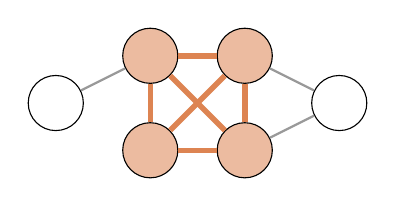
\begin{tikzpicture}
        \node[pick] (a) at (0,1.2) {};
        \node[pick] (b) at (1.2,1.2) {};
        \node[pick] (c) at (1.2,0) {};
        \node[pick] (d) at (0,0) {};
        \node[vtx] (e) at (2.4,0.6) {};
        \node[vtx] (f) at (-1.2,0.6) {};
        \draw[hot] (a)--(b)--(c)--(d)--(a); \draw[hot] (a)--(c);
        \draw[hot] (b)--(d);
        \draw[edg] (b)--(e)--(c); \draw[edg] (f)--(a);
      \end{tikzpicture}\\[2pt]
      \small A clique of size 4.
      \end{center}
    \end{column}
  \end{columns}

  \medskip
  Independent set: \alert{no} pair adjacent. Clique: \alert{every} pair
  adjacent. Opposites!
\end{frame}

\begin{frame}{The Complement Graph}
  The \alert{complement} $\bar{G}$ has the same vertices, and an edge exactly
  where $G$ has \alert{none}. Computing it takes $O(n^2)$ time.

  \begin{columns}[c]
    \begin{column}{0.48\textwidth}
      \begin{center}
      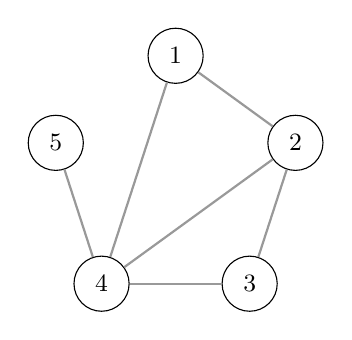
\begin{tikzpicture}
        \pentagon{vtx, onslide=<2->{pick}}{vtx}{vtx, onslide=<2->{pick}}%
                 {vtx}{vtx, onslide=<2->{pick}}
        \draw[edg] (v1)--(v2); \draw[edg] (v2)--(v3); \draw[edg] (v3)--(v4);
        \draw[edg] (v4)--(v5); \draw[edg] (v2)--(v4); \draw[edg] (v1)--(v4);
      \end{tikzpicture}\\[2pt]
      $G$
      \end{center}
    \end{column}
    \begin{column}{0.48\textwidth}
      \begin{center}
      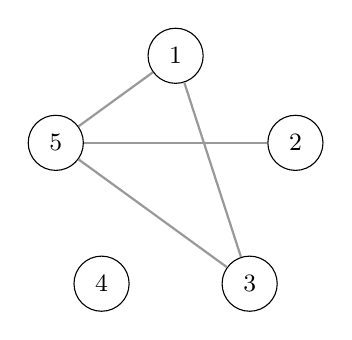
\begin{tikzpicture}
        \pentagon{vtx, onslide=<2->{pick}}{vtx}{vtx, onslide=<2->{pick}}%
                 {vtx}{vtx, onslide=<2->{pick}}
        \draw[edg] (v2)--(v5);
        \draw[edg, onslide=<2->{hot}] (v1)--(v3);
        \draw[edg, onslide=<2->{hot}] (v1)--(v5);
        \draw[edg, onslide=<2->{hot}] (v3)--(v5);
      \end{tikzpicture}\\[2pt]
      $\bar{G}$
      \end{center}
    \end{column}
  \end{columns}

  \medskip
  \onslide<2->{$\{1, 3, 5\}$ is an independent set in $G$ and a clique in
  $\bar{G}$.}
\end{frame}

\begin{frame}{Independent Set $\le_p$ Clique}
  \begin{block}{Observation}
    $S$ is an independent set in $G$ $\iff$ $S$ is a clique in $\bar{G}$.
  \end{block}

  \textbf{Proof.} For distinct $u, v \in S$:
  $\{u, v\} \notin E \iff \{u, v\} \in \bar{E}$. So ``no pair is an edge of
  $G$'' is the same as ``every pair is an edge of $\bar{G}$''.
  \hfill $\square$

  \pause
  \begin{block}{Theorem}
    Clique is NP-complete.
  \end{block}

  \textbf{Proof.} Clique $\in \mathbf{NP}$ (above). Reduction: map an
  Independent Set instance $(G, k)$ to the Clique instance $(\bar{G}, k)$,
  in $O(n^2)$ time. By the observation, $G$ has an independent set of size
  $\ge k$ $\iff$ $\bar{G}$ has a clique of size $\ge k$. Independent Set is
  NP-complete, so Clique is NP-hard. \hfill $\square$
\end{frame}

% =========================================================================
\section{Vertex Cover}

\begin{frame}{Vertex Cover}
  A \alert{vertex cover} of $G = (V, E)$ is a set $C \subseteq V$ that
  touches every edge: for every $\{u, v\} \in E$, $u \in C$ or $v \in C$.

  \begin{columns}[c]
    \begin{column}{0.55\textwidth}
      \begin{block}{Vertex Cover}
        Given $G$ and $k$, does $G$ have a vertex cover of size $\le k$?
      \end{block}

      \medskip
      \textbf{In NP.} Certificate: the set $C$. Check $|C| \le k$ and scan
      every edge, $O(n + m)$ time.

      \medskip
      \small Think: place guards at vertices so every road (edge) is
      watched.
    \end{column}
    \begin{column}{0.4\textwidth}
      \begin{center}
      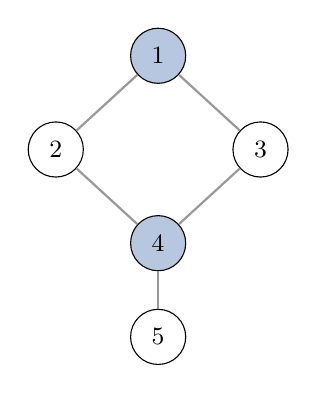
\begin{tikzpicture}[yscale=0.85]
        \node[cov] (1) at (0,2)    {1};
        \node[vtx] (2) at (-1.3,0.6) {2};
        \node[vtx] (3) at (1.3,0.6)  {3};
        \node[cov] (4) at (0,-0.8) {4};
        \node[vtx] (5) at (0,-2.2) {5};
        \draw[edg] (1)--(2); \draw[edg] (1)--(3); \draw[edg] (2)--(4);
        \draw[edg] (3)--(4); \draw[edg] (4)--(5);
      \end{tikzpicture}\\[2pt]
      \small $\{1, 4\}$ (blue) covers all 5 edges.
      \end{center}
    \end{column}
  \end{columns}
\end{frame}

\begin{frame}{Covers and Independent Sets Are Complements}
  \begin{columns}[c]
    \begin{column}{0.6\textwidth}
      \begin{block}{Observation}
        $S$ is an independent set $\iff$ $V \setminus S$ is a vertex cover.
      \end{block}

      ($\Rightarrow$) Take any edge $\{u, v\}$. Not both ends are in $S$, so
      at least one is in $V \setminus S$.

      \medskip
      ($\Leftarrow$) If some edge had both ends in $S$, neither end would be
      in $V \setminus S$, which would then miss that edge.
      \hfill $\square$
    \end{column}
    \begin{column}{0.35\textwidth}
      \begin{center}
      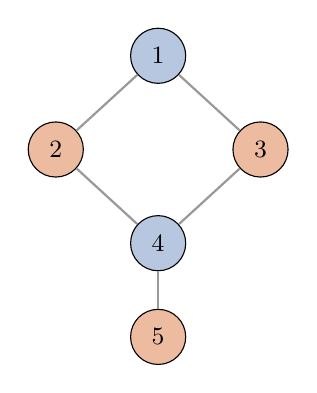
\begin{tikzpicture}[yscale=0.85]
        \node[cov] (1) at (0,2)    {1};
        \node[pick] (2) at (-1.3,0.6) {2};
        \node[pick] (3) at (1.3,0.6)  {3};
        \node[cov] (4) at (0,-0.8) {4};
        \node[pick] (5) at (0,-2.2) {5};
        \draw[edg] (1)--(2); \draw[edg] (1)--(3); \draw[edg] (2)--(4);
        \draw[edg] (3)--(4); \draw[edg] (4)--(5);
      \end{tikzpicture}\\[2pt]
      \small cover $\{1, 4\}$ (blue),\\ independent set $\{2, 3, 5\}$
      (orange)
      \end{center}
    \end{column}
  \end{columns}
\end{frame}

\begin{frame}{Independent Set $\le_p$ Vertex Cover}
  \begin{block}{Theorem}
    Vertex Cover is NP-complete.
  \end{block}

  \textbf{Proof.} Vertex Cover $\in \mathbf{NP}$ (above). Reduction: map an
  Independent Set instance $(G, k)$ to the Vertex Cover instance
  $(G, n - k)$: the same graph, with target $n - k$.

  \medskip
  By the observation,
  \[
    G \text{ has an independent set of size } \ge k
    \iff G \text{ has a vertex cover of size } \le n - k.
  \]
  Independent Set is NP-complete, so Vertex Cover is NP-hard.
  \hfill $\square$

  \pause
  \bigskip
  \textbf{Note.} \emph{Minimum} vertex cover and \emph{maximum} independent
  set are the same problem in disguise:
  $\text{min cover} = n - \text{max independent set}$.
\end{frame}

% =========================================================================
\begin{frame}{The Reductions So Far}
  \begin{center}
  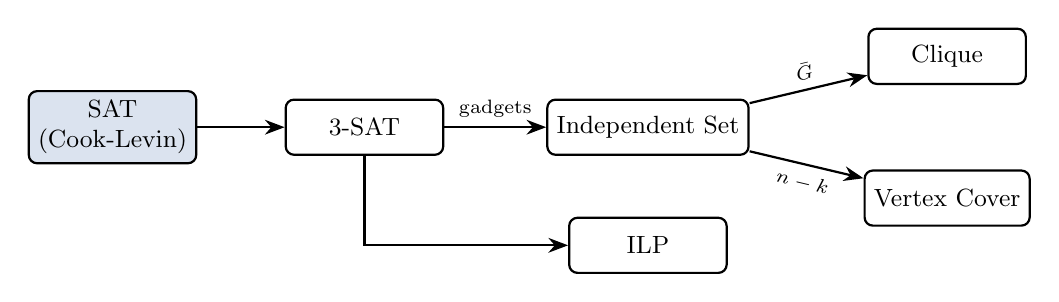
\begin{tikzpicture}[box/.append style={minimum width=20mm}]
    \node[box, fill=mLightBlue!20] (cl) at (0,0) {SAT\\(Cook-Levin)};
    \node[box] (sat) at (3.2,0) {3-SAT};
    \node[box] (is) at (6.8,0) {Independent Set};
    \node[box] (cq) at (10.6,0.9) {Clique};
    \node[box] (vc) at (10.6,-0.9) {Vertex Cover};
    \node[box] (ilp) at (6.8,-1.5) {ILP};
    \draw[arr] (cl) -- (sat);
    \draw[arr] (sat) -- node[above, font=\scriptsize] {gadgets} (is);
    \draw[arr] (sat) |- (ilp);
    \draw[arr] (is) -- node[above, sloped, font=\scriptsize] {$\bar{G}$} (cq);
    \draw[arr] (is) -- node[below, sloped, font=\scriptsize] {$n - k$} (vc);
  \end{tikzpicture}
  \end{center}

  \bigskip
  \begin{itemize}
    \item Every problem here is NP-complete, so each reduces to every other
          one (through Cook-Levin, if not directly).
    \item Many more are known: Hamiltonian Cycle, 3-Coloring, Subset Sum,
          Traveling Salesman, \ldots{} (Karp's 21 problems, 1972).
    \item The more problems we know are NP-complete, the easier it is to find
          one close to a new problem to reduce from.
  \end{itemize}
\end{frame}

% =========================================================================
\begin{frame}{Exercise}
  \begin{columns}[c]
    \begin{column}{0.3\textwidth}
      \begin{center}
      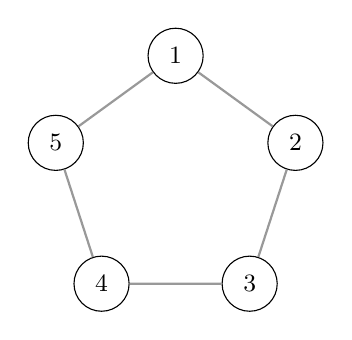
\begin{tikzpicture}
        \pentagon{vtx}{vtx}{vtx}{vtx}{vtx}
        \draw[edg] (v1)--(v2)--(v3)--(v4)--(v5)--(v1);
      \end{tikzpicture}\\[2pt]
      \small The 5-cycle $C_5$
      \end{center}
    \end{column}
    \begin{column}{0.65\textwidth}
      \begin{enumerate}
        \item For $C_5$, find a maximum independent set, a minimum vertex
              cover, and a maximum clique of $\bar{C_5}$. Check the
              relations from today.
        \item Give a direct reduction Vertex Cover $\le_p$ Clique.
        \item A friend shows Vertex Cover $\le_p$ ILP. Is that a new proof
              that ILP is NP-hard?
        \item A friend shows ILP $\le_p$ Vertex Cover. Does that show ILP is
              NP-hard?
      \end{enumerate}
    \end{column}
  \end{columns}
\end{frame}

\begin{frame}{Solution}
  \begin{columns}[c]
    \begin{column}{0.3\textwidth}
      \begin{center}
      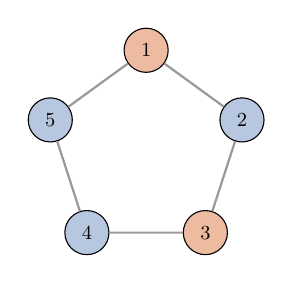
\begin{tikzpicture}[scale=0.8, every node/.append style={transform shape}]
        \pentagon{pick}{cov}{pick}{cov}{cov}
        \draw[edg] (v1)--(v2)--(v3)--(v4)--(v5)--(v1);
      \end{tikzpicture}\\[2pt]
      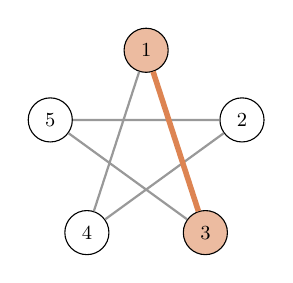
\begin{tikzpicture}[scale=0.8, every node/.append style={transform shape}]
        \pentagon{pick}{vtx}{pick}{vtx}{vtx}
        \draw[edg] (v1)--(v4)--(v2)--(v5)--(v3);
        \draw[hot] (v1)--(v3);
      \end{tikzpicture}\\[2pt]
      \small $C_5$ and $\bar{C_5}$
      \end{center}
    \end{column}
    \begin{column}{0.66\textwidth}
      \small
      \textbf{(a)} Max independent set $\{1, 3\}$, size 2 (three of five
      vertices on a 5-cycle always include two neighbors). Min cover
      $\{2, 4, 5\}$, size $3 = 5 - 2$. $\bar{C_5}$ is again a 5-cycle; its
      max clique $\{1, 3\}$ has size 2, the same as the max independent set
      of $C_5$.

      \medskip
      \textbf{(b)} $(G, k) \mapsto (\bar{G}, n - k)$: $G$ has a cover of size
      $\le k$ $\iff$ an independent set of size $\ge n - k$ $\iff$
      $\bar{G}$ has a clique of size $\ge n - k$.

      \medskip
      \textbf{(c)} Yes. Vertex Cover is NP-complete, so reducing it to ILP
      shows ILP is NP-hard (another route besides 3-SAT).

      \medskip
      \textbf{(d)} No, wrong direction. It shows ILP is no harder than Vertex
      Cover, which says nothing about ILP being hard.
    \end{column}
  \end{columns}
\end{frame}

% =========================================================================
\begin{frame}{Summary}
  \begin{itemize}
    \item \textbf{Clique}: every pair adjacent. Independent sets of $G$ are
          exactly the cliques of $\bar{G}$, so $(G, k) \mapsto (\bar{G}, k)$.
    \item \textbf{Vertex Cover}: touch every edge. $S$ is independent
          $\iff$ $V \setminus S$ is a cover, so $(G, k) \mapsto (G, n - k)$.
    \item Both are in NP, so both are NP-complete.
    \item To prove a new problem hard, reduce \alert{from} a known
          NP-complete problem that looks similar, and check both directions
          of the ``if and only if''.
  \end{itemize}
\end{frame}

\end{document}
